%%%%%%%%%%%%%%%%%%%%%%%%%%%%%%%%%%%%%%%%%%%%%%%%%%%
%% Éléments flottants
%%%%%%%%%%%%%%%%%%%%%%%%%%%%%%%%%%%%%%%%%%%%%%%%%%%
%%%%%%%%%%%%%%%%%%
\section{Méthodologie de gestion de projets}
\addcontentsline{toc}{subsection}{Introduction}
\subsection*{Introduction}
Dans ce chapitre, nous aborderons les aspects de la gestion de projet, de la composition des équipes, des outils et des méthodes de développement de logiciels adoptés par Cegedim SRH.
\subsection{Étude préliminaire}
\subsubsection{Origine du génie logiciel}
\begin{beware}[title=Définition : ]
Le génie logiciel est la science de l'ingénieur qui s'intéresse aux procédés scientifiques de construction et d'entretien des logiciels, et bien évidemment à la « matière » même de cette construction : d'abord les programmes eux-mêmes, les fichiers et bases de données, les scripts de paramétrage nécessaires à l'exécution du programme, puis tout ce qui gravite autour (spécification de besoins et exigences des futurs utilisateurs, conception, tests, documentation pour les mainteneurs, le support technique et les usagers)\cite{origine_gl1}.
\end{beware}

À la fin des années 50, l’informatique est devenue de plus en plus populaire et s’est étendue à d’autres disciplines. Ceci en raison de l’impulsion des grands projets spatiaux et militaires, grands consommateurs de logiciels et imposant des exigences de qualité et de sûreté de fonctionnement et du fait que les informaticiens du génie logiciel étaient plus enclins et plus à même de développer des outils logiciels d’aide à la conduite des activités.\\

En octobre 1968, l'OTAN a organisé une première conférence, à Partenkirchen en Allemagne, sur l’industrialisation de l’élaboration du logiciel. C’est à cette occasion qu'est forgée l’expression « Software Engineering » pour donner une tournure délibérément industrielle au propos\cite{origine_gl3}.\\

À la fin des années 60, les grands systèmes commerciaux ont démontré qu'il était difficile d'adapter à grande échelle les principes qui avaient été adéquats jusque là. Les grands projets dépassaient les budgets et les délais, ce fût alors « the software crisis » la crise du logiciel\cite{origine_gl2}.\\

La conférence de l'OTAN a été immédiatement suivie par de nombreuses autres conférences portant sur des thèmes liés au génie logiciel, tels que la fiabilité des logiciels, le test du logiciel, la spécification du logiciel, la maintenance du logiciel, etc.

En 1975 s'est tenue la première conférence véritablement dédiée à l’ensemble du génie logiciel, accompagnée d'une exposition de premiers outils, notamment pour l’aide au test. Depuis, l’IEEE tient une rencontre annuelle internationale. Cette première conférence a correspondu à la création, au sein de l’IEEE, d’un comité technique dédié au génie logiciel, animateur d’une série de conférences et ateliers récurrents et éditeur de deux revues dédiées au génie logiciel\cite{origine_gl3}.
\subsubsection{Comparaison des différentes méthodes de développement}
\subsubsubsection{Les approches traditionnelles}
Dans une approche traditionnelle, le cycle de vie d'un logiciel passe par quatre phases principales : \textbf{initiation}, \textbf{développement}, \textbf{déploiement} et \textbf{exploitation}.
\begin{itemize}
    \item \textbf{L'initiation} vise à déterminer la mission du système et à effectuer des travaux exploratoires permettant de vérifier la pertinence du projet.
    \item \textbf{Le développement} est la phase qui prend en charge la réalisation du logiciel. Elle précise les besoins, réalise le produit et valide son fonctionnement.
    \item \textbf{Le déploiement} rend le produit accessible à ses utilisateurs, par la mise en service du logiciel dans son environnement de production.
    \item \textbf{L’exploitation} est la période de vie utile du produit au cours de laquelle des améliorations peuvent être apportées au produit.
\end{itemize}

% Un ensemble d’éléments est nécessaire à un projet conduit par une approche traditionnelle. 
% La table ~\ref{tab:trad} résume les phases et les principales tâches qu’elles regroupent.

% \begin{longtblr}[caption={Description des étapes du cycle de vie logiciel dans une apporche traditionnelle},label={tab:trad}]{
%     hlines = {0.25pt,azure6},
%     vlines = {0.25pt,azure6},
%     row{odd} = {bg=azure9!10!white},
%     colsep=4pt,
%     rowsep=4pt,
% 	colspec={cX},
%     rowspec={Q[m] Q[m] Q[m] Q[m] Q[m] Q[m] Q[m] Q[m] Q[m] Q[m] Q[m] Q[m] Q[m] Q[m] Q[m] Q[m] Q[m] Q[m] Q[m] Q[m] Q[m]},
%     cell{1}{2} = {c},
%     cell{2}{1} = {c=2}{c,azure7},
%     cell{5}{1} = {c=2}{c,azure7},
%     cell{12}{1} = {c=2}{c,azure7},
%     cell{18}{1} = {c=2}{c,azure7},
% }
% \textbf{Étapes}&\textbf{Description}\\
% \textbf{Initiation}\\
% Étude de faisabilité
%  & L'ÉTUDE DE FAISABILITÉ produit un document qui analyse les besoins et définit le mandat et les limites du système.\\
%  Planification du projet
% & 
% LE PLAN DE PROJET présente à travers le temps les différentes phases du projet, il
% précise ses ressources, son délai et son coût.\\
% \textbf{Développement}\\
% {Analyse et spécifications
% \\des besoins}
% & 
% LES SPÉCIFICATIONS REQUISES analysent et précisent les qualités internes requises pour juger de la conformité du produit. 
% \\
% {Spécification du design
% \\(Architecture)}
% &  LES SPÉCIFICATIONS DU DESIGN, correspondent à la décomposition en modules et les relations qu’ils ont entre eux.\\
% Analyse fonctionnelle
% &  L’ANALYSE FONCTIONNELLE détaille les unités de programmation à leur plus bas niveau, avant d’être codé. L’ensemble des éléments doit précisément y être spécifié. On y retrouve les maquettes d’écran, les données exploitées et le détail des algorithmes.\\
% {Programmation et tests
% \\unitaires}&La programmation réalise Le Code Source, qui est le livrable de cette étape. UN PLAN DE TESTS UNITAIRES doit aussi être produit pour valider le code.\\
% {Intégrations et tests
% \\systèmes}& L’intégration consiste à valider l’interaction des unités de programmation ensemble.
% UN PLAN DES TESTS SYSTÈMES prévoit la vérification des échanges entre les unités et les modules du système. Les interfaces modulaires sont testées à ce niveau.\\
% Documentation & La documentation explique comment exploiter l’application. La DOCUMENTATION TECHNIQUE est destinée à l’administration du système et la DOCUMENTATION DIDACTIQUE est destinée aux utilisateurs, elle est utilisée lors des sessions de formation. \\
% \textbf{Déploiement}\\
% Plan de déploiement & L’implantation est l’étape de livraison du produit au client. Le logiciel doit être installé sur les machines de production réelle. LE PLAN D’IMPLANTATION guide les étapes à suivre pour procéder à cette mise en service.\\
% Formation & Les utilisateurs doivent être formés sur le nouveau système, afin qu’ils connaissent les fonctionnalités disponibles dans leur nouveau système. LE PLAN DE FORMATION détaille la stratégie et les moyens utilisés.\\
% Conversion de données & Cette étape sert à alimenter le nouveau système à partir de données existantes. Celles-ci doivent être converties dans un nouveau format. UN PLAN DE CONVERSION doit être produit afin de spécifier les interfaces d’importation et l’exportation des données existantes.\\
% Tests d'acceptation & Les tests d’acceptation sont réalisés par les pilotes ou les utilisateurs, afin de d’approuver le système. UNE LISTE DES DEMANDES DE CORRECTIONS est rédigée dans le but de corriger les éléments non conformes aux attentes du client.\\
% Vérification posthume & 
% Lors de la fermeture du projet de développement, une vérification posthume révise le déroulement des différentes étapes. LE RAPPORT DE FIN DE PROJET explique les difficultés rencontrées et les bonnes pratiques à retenir.\\
% \textbf{Exploitation}\\
% {Suivi Opérationnel 
% \\et support} & Le suivi opérationnel assure le fonctionnement du système. Des éléments de surveillance permettent de contrôler le fonctionnement. Le support consiste à répondre aux questions et à compléter la formation auprès de l’équipe en charge de l’exploitation ou des utilisateurs.\\
% Maintenance & La maintenance du système permet de corriger les erreurs de conception et de
% compléter ou d’ajouter des fonctionnalités\\

% {Décisions récurrentes :
% \\Continuer – Refaire -
% \\Terminer} & Le système doit être évalué de manière récurrente pour confirmer sa pertinence. À travers le temps, de nouvelles opportunités peuvent comporter suffisamment d’avantages pour abandonner un système désuet. 

% \end{longtblr}

\subsubsubsection{Les méthodes agiles}
Une méthode agile est une approche itérative et incrémentale, qui est menée dans un esprit collaboratif, avec juste ce qu’il faut de formalisme. Elle génère un produit de haute qualité tout en prenant en compte l’évolution des besoins des clients\cite{agile1}.\\

Le Manifeste Agile déclare quatre valeurs dans toute approche agile. Chaque méthode adopte ensuite sa propre terminologie et recommande un certain nombre de pratiques. Les quatre valeurs du Manifeste sont\cite{agile1, agile4} :
\begin{itemize}
    \item Les individus et leurs interactions avant les processus et les outils. 
    \item Des fonctionnalités opérationnelles avant la documentation.
    \item Collaboration avec le client plutôt que contractualisation des relations. 
    \item Acceptation du changement plutôt que conformité aux plans.
\end{itemize}

\subsubsubsection{Synthèse}
Bien que les approches traditionnelles présentent divers avantages, elles ont aussi certaines limites, en particulier dans les environnements évolutifs. En effet, les environnements évolutifs nécessitent des adaptations constantes. Avec une planification rigoureuse, il est difficile d’apporter des changements à cause de leurs impacts, et plus un changement est fait tard, plus il est coûteux. Cette situation tardive exige de modifier l'enchaînement des étapes antérieures et seuls les changements les plus importants seront opérés.\\

% Certains projets peuvent requérir moins d’effort de gestion. Les suivis et les rapports alourdissent la charge administrative. Les communications écrites sont coûteuses et longues à produire. Il faut tenir compte de l’ampleur et de la complexité du projet. Si le produit est livré dans un délai important, il est possible que la situation du client ait évolué et que l’on soit appelé à modifier le système.\\

Selon une nouvelle étude menée par Organize Agile\cite{organize_agile} auprès de professionnels de 19 pays, près de la moitié des organisations utilisent des méthodes agiles depuis trois ans ou plus. Ces entreprises utilisent principalement Agile comme méthodologie pour leurs programmes de réforme - connus sous le nom de transformations agiles. Il s'agit de grands changements organisationnels qui adoptent le travail agile au sein de petites équipes multidisciplinaires qui s'attachent à fournir des résultats de manière rapide, expérimentale et itérative, ce qui révèle l'impact positif de ces méthodes sur les flux de travail des projets informatiques à l'échelle mondiale. Au Maroc, selon un rapport d'étude publié en 2011 impliquant 48 organisations participantes représentant les secteurs privé et public a révélé que le taux de satisfaction de la maîtrise d'ouvrage est plus élevé pour les DSI adoptant une des méthodes agiles ce qui démontre leur pragmatisme et leur efficacité par rapport aux méthodes traditionnelles en cascade\cite{badr_2011}.\\

Les approches agiles et traditionnelles convergent et divergent sur différents aspects. L’expérience de l’équipe peut faire diminuer les risques et contribuer à minimiser les exigences de suivi. Les approbations et le manque d’autonomie des équipes peuvent ralentir le projet. Une organisation peu hiérarchisée, ayant une culture collégiale, intégrera difficilement une structure traditionnelle.\\
\subsection{Conduite de projet}
\subsubsection{Modèle de livraison}
Aujourd'hui, Cegedim adopte une approche de livraison agile que tout projet est censé suivre. Le schéma ci-dessous montre les différentes phases de ce modèle (voir figure  ~\ref{fig:delivery}) :
\begin{figure}[H]
    \begin{center}
        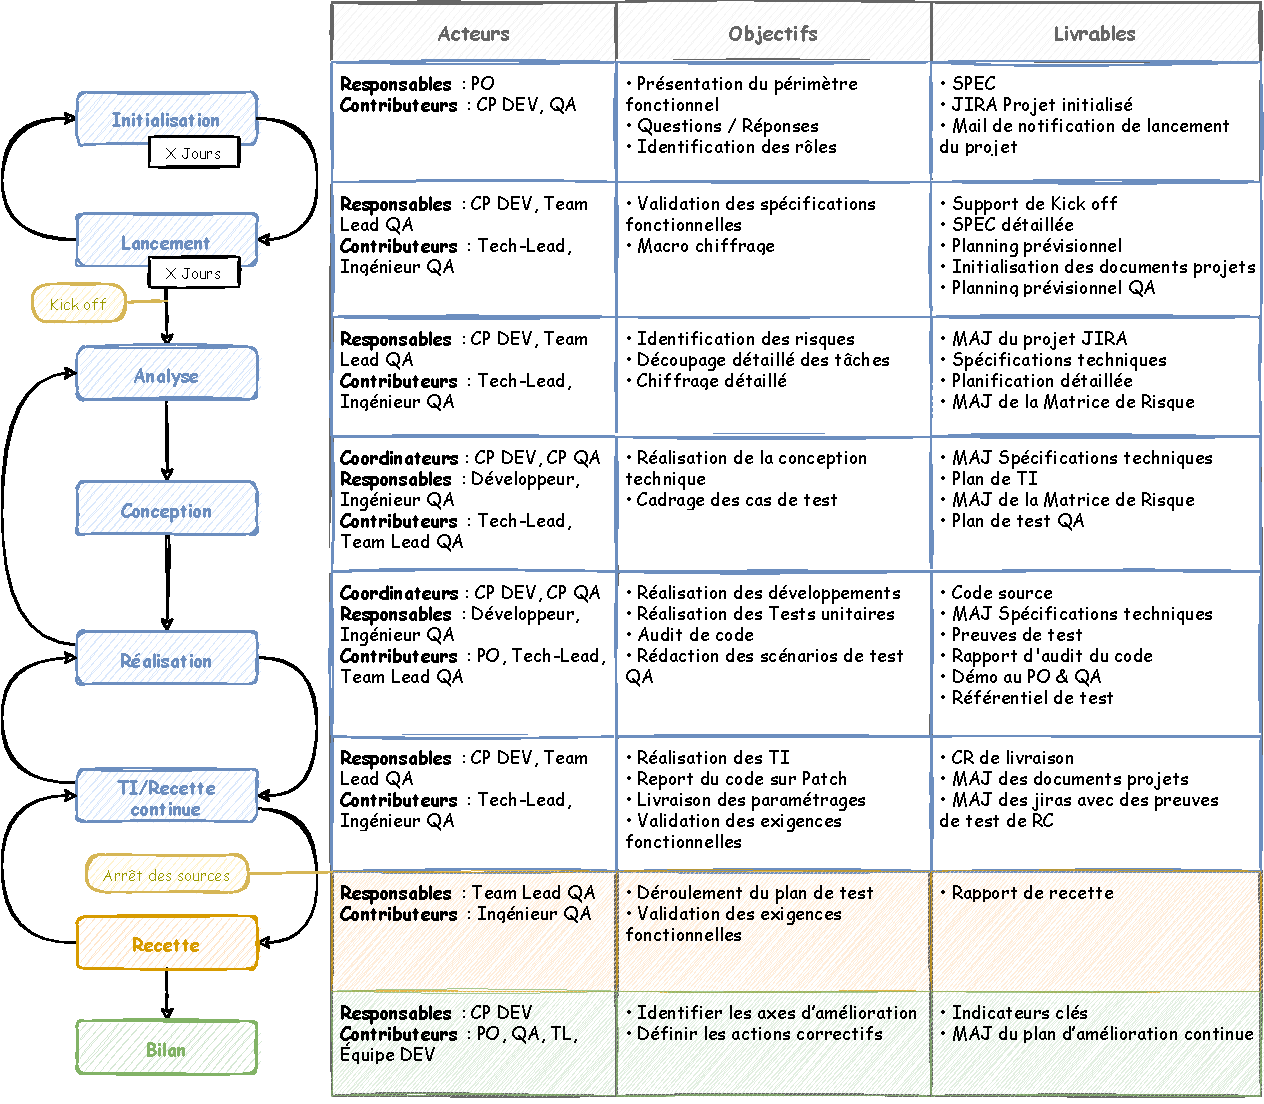
\includegraphics[width=\linewidth]{images/sec3/deliveryprocess.pdf}
        \caption{Modèle de livraison}
        \label{fig:delivery}
    \end{center}
\end{figure}
Les acteurs impliqués dans le processus de livraison peuvent être répartis en deux grandes divisions (voir figure \ref{fig:devetqa}, tableaux \ref{tab:dev} et \ref{tab:qa}) :
\begin{figure}[H]
    \centering
    \begin{subfigure}[t]{0.53\textwidth}
        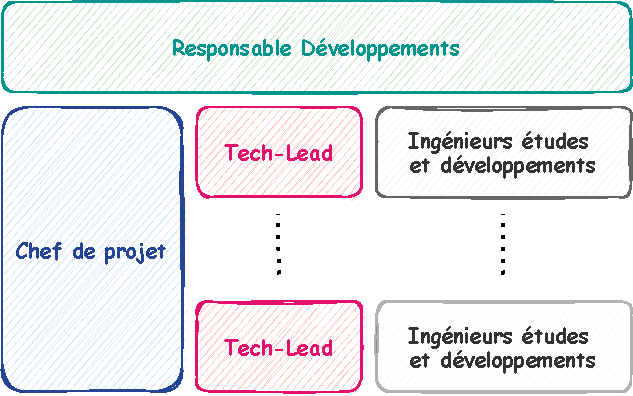
\includegraphics[width=\textwidth,]{images/sec3/organigrammedev.pdf}
        \caption{Organisation cible dév}
        \label{fig:subfig1}
    \end{subfigure}
    \hfill
    \begin{subfigure}[t]{0.39\textwidth}
        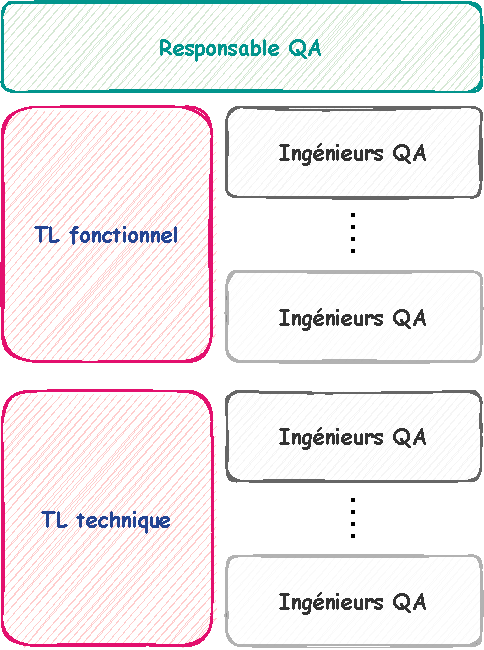
\includegraphics[width=\textwidth]{images/sec3/organigrammeqa.pdf}
        \caption{Organisation cible QA}
        \label{fig:subfig2}
    \end{subfigure}
    \caption{Modèle organisationnel visé pour les équipes de développement et de QA}
    \label{fig:devetqa}
\end{figure}
Le tableau suivant (\ref{tab:dev}) décrit les différentes activités et tâches confiées aux membres de l'équipe de développement impliqués dans le processus de livraison :
\begin{longtblr}[caption={Responsabilités et missions des différents acteurs de l'équipe de dév}, label={tab:dev}]{
    hlines = {0.25pt,azure6},
    vlines = {0.25pt,azure6},
    colsep=4pt,
    rowsep=4pt,
	colspec={X},
}
\textbf{Équipe de développement}
\\
\begin{minipage}{\linewidth}
{ \color{actGreen}
\textbf{Responsable Développements}\\
}
 \begin{itemize}
    \item Accompagner le chef de projet dans la gestion des projets.
    \item Produire des indicateurs sur l’activité de développement.
    \item Suivi des risques et gestion des alertes.
    \item Travailler en collaboration avec les autres responsables de division.\\
 \end{itemize}
\end{minipage}
\\
\begin{minipage}{\linewidth}
    {
        \color{actBlue}\textbf{Chef de projet}\\
    }
    \begin{itemize}
        \item Valider les spécifications fonctionnelles.
        \item Assurer le suivi du processus de livraison et des indicateurs clés.
        \item Élaboration du plan de charge et planification des équipes.
        \item Garant des engagements (Qualité, Délai, Coût).\\
    \end{itemize}
\end{minipage}\\
\begin{minipage}{\linewidth}
    {
        \color{actPink}\textbf{Tech-Lead}\\
    }
    \begin{itemize}
        \item Responsable de la qualité technique (Audit, conception, etc.).
        \item Responsable des bonnes pratiques de développement.
        \item Encadrement et assistance technique.
        \item Participer aux développements.
        \item Assister le chef de projet pour les estimations de charge.\\
    \end{itemize}
\end{minipage}\\
\begin{minipage}{\linewidth}
    {
        \textbf{Ingénieur étude et développement}\\
    }
    \begin{itemize}
        \item Corriger les anomalies et développer de nouveaux modules.
        \item Respecter les bonnes pratiques de développement.
        \item Participer à la définition de la couverture de tests techniques.
        \item Rédiger des documents techniques.\\
    \end{itemize}
\end{minipage}
\end{longtblr}
Le tableau suivant (\ref{tab:qa}) décrit les différentes activités et tâches assignées aux membres de l'équipe d'assurance qualité (QA) participant au processus de livraison :
\begin{longtblr}[caption={Responsabilités et missions des différents acteurs de l'équipe QA}, label={tab:qa}]{
    hlines = {0.25pt,azure6},
    vlines = {0.25pt,azure6},
    colsep=4pt,
    rowsep=4pt,
	colspec={X},
}
\textbf{Équipe QA}\\

\begin{minipage}{\linewidth}
{\color{actGreen}
\textbf{Responsable QA}\\
}
 \begin{itemize}
     \item Établir et piloter une stratégie de test.
     \item Accompagner le Team Lead dans la gestion des projets.
     \item Contribuer à l'amélioration des processus de test.
     \item Produire des indicateurs sur l’activité de testing.
     \item Suivi des risques et gestion des alertes.
     \item Travailler en collaboration avec les autres responsables de division.\\
 \end{itemize}
\end{minipage}\\
\begin{minipage}{\linewidth}
    {
    \color{actBlue}\textbf{TL fonctionnel/technique}\\
    }
    \begin{itemize}
        \item Responsable du suivi du processus de livraison et des indicateurs clés.
        \item Élaboration du plan de charge et la planification des équipes.
        \item Accompagner et suivre les testeurs dans la mise en place des bonnes pratiques et des outils.
        \item Accompagner les ingénieurs QA dans l'élaboration des plans de test.
        \item Réaliser le bilan des activités.
        \item Accompagner l'intégration des nouveaux arrivants et veiller à la montée en compétence des équipes.
        \item Participer aux activités de test.\\
    \end{itemize}
    \end{minipage}\\
    \begin{minipage}{\linewidth}
    {
        \textbf{Ingénieur QA}\\
    }
    \begin{itemize}
        \item Formaliser des scénarios de test fonctionnels et automatisés.
        \item Valider et vérifier le développement de l’application.
        \item Respecter les bonnes pratiques de testing.
        \item Rédiger des documents fonctionnels.\\
    \end{itemize}
\end{minipage}
\end{longtblr}

\subsubsection{Déroulement de projets - Méthode SCRUM}
Depuis 2019, les projets de R\&D ont progressivement passés en mode Agile. Ils utilisent la partie Agile de JIRA (catégorie Software).
Le mode Agile permet de gérer les projets en mode Scrum ou Kanban. Pour l'instant, Cegedim SRH utilise le mode Scrum.
\subsubsubsection{L'équipe Agile}
L'équipe Agile est une équipe qui entend être totalement autonome. Elle rassemble toutes les compétences nécessaires pour faire évoluer le produit. Le maître mot d'une équipe agile est la coopération. En effet, les membres de l'équipe ne travaillent pas séparément sur les fonctionnalités qui leur sont assignées, mais ensemble, y compris pour l'identification, la définition, la réalisation et les tests des fonctionnalités.

Les capacités d’écoute et d’entraide de l’équipe facilitent la montée en compétence. Chaque membre devient petit à petit plus ou moins polyvalent et en capacité d'aider les autres dans la réalisation des différentes fonctionnalités. L’équipe devient donc de plus en plus performante et efficace, tout en améliorant également le ressenti et les conditions de travail de chacun.
\begin{beware}
Une équipe Agile est en perpétuelle progression et évolution.
\end{beware}
Il n'y a pas de composition type pour une équipe Agile. Celle-ci dépend totalement du produit à réaliser. Certains rôles clefs sont néanmoins nécessaires au bon fonctionnement de l'équipe.
 La composition d'une équipe Agile au sein de la R\&D SRH suivra à minima le modèle suivant :

\begin{itemize}
\item \textbf{Equipe Agile R\&D}
\begin{itemize}
    \item 1 Product Owner ;
    \item 1 Scrum Master (optionnel mais conseillé) ;
    \item X développeurs (il est recommandé d'avoir +2) ;
    \item 1 QA (optionnel) ;
    \item X testeur(s)
\end{itemize}
\end{itemize}
Bien entendu, selon les produits, cette structure sera susceptible d'évoluer.
\subsubsubsection{Le Sprint}
Le Sprint agile est le cœur de la méthode SCRUM. Tous les développements sont réalisés de manière incrémentale au sein des Sprints. Un périmètre de développement - l'objectif du Sprint - est défini au début du Sprint lors du \textbf{Sprint Planning} avec la liste des \textbf{User Stories} à traiter pendant le Sprint.\\

À la conclusion d'un Sprint, le bilan est réalisé lors du \textbf{Sprint Review}, puis un nouveau cycle démarre avec un nouveau Sprint. La périodicité d'un Sprint dépendra de l'équipe Agile, mais sera généralement entre 2 et 4 semaines.

\subsubsubsection{Les Rituels}
Les rituels (ou cérémonies) sont des réunions de travail et de suivi qui viennent rythmer un Sprint. Chaque réunion joue un rôle précis dans le Sprint et correspond à une temporalité particulière.
\begin{itemize}
    \item \textbf{\underline{Sprint Planning}} : Le Sprint Planning est la réunion de lancement d'un Sprint. Au début de chaque Sprint, le Product Owner présente les User Stories qu'il souhaiterait intégrer au Sprint. Les User Stories sont examinées une par une dans l'ordre de priorité du Backlog jusqu'à ce que le Sprint soit complet en termes de vélocité.\\
    L'examen d'une User Story suit les étapes suivantes :
\begin{itemize}
    \item Lecture de la User Story par le Product Owner.
    \item Questions des développeurs (optionnel).
    \item Poker Planning : les développeurs estiment le temps nécessaire pour le développement de la User Story en votant chacun pour une durée. Pour passer à l'étape suivante, il doit y avoir un consensus sur l'estimation. Si tel n'est pas le cas, les développeurs ayant donné les estimations extrêmes doivent s'expliquer et un nouveau vote est réalisé.
    \item Intégration de la User Story au Sprint : passage en "A faire" dans le Board de l'équipe.
\end{itemize}
\begin{beware}[borderline west={5pt}{0pt}{olive3}, coltitle={olive3}, title=Note : ]
    Le Sprint Planning a lieu impérativement le premier jour du Sprint, de préférence le matin afin d'optimiser un maximum le temps de travail de l'équipe sur le Sprint.
\end{beware}
\begin{beware}[title=Remarque : ]
À l'étape "Questions", si les développeurs ne comprennent pas ce qu'il faut faire, la User Story est replacée dans le Backlog en vue d'être détaillée plus avant par le Product Owner.
De même, lors du "Poker Planning", si ces derniers n'arrivent pas à se mettre d'accord sur une estimation de temps commune.
\end{beware}

\item \textbf{\underline{Daily Stand-Up Meeting}} : Le Daily Stand-up meeting est une réunion quotidienne très courte (entre 5 et 15 minutes) à heure et lieu fixes qui rassemble l'ensemble des membres de l'équipe Agile où chaque membre de l'équipe prend la parole à tour de rôle. Chacun doit expliquer ce qu'il a fait depuis l'itération précédente du Stand-up meeting ou le Sprint Planning et ce qu'il prévoit faire jusqu'au prochain Stand-up meeting. 
\begin{beware}[borderline west={5pt}{0pt}{red}, coltitle={red}, title=Remarque : ]
Le temps de parole de chacun ne doit généralement pas dépasser deux minutes.
\end{beware}
Le Stand-up meeting a pour but de favoriser la circulation des informations au sein de l'équipe. Elle permet à l'ensemble de l'équipe d'avoir une vue complète de l'avancée des tâches et d'identifier d'éventuels points de blocages. Ces échanges dynamiques contribuent également à la cohésion et l'implication de l'équipe.
\begin{beware}[borderline west={5pt}{0pt}{red}, coltitle={red}, title=Attention : ]
\begin{itemize}
    \item La tenue du Stand-up meeting n'est pas facultative.
    \item Si un sujet est susceptible de déborder, il doit être traité en dehors du cadre du Stand-up meeting avec les membres concernés.
\end{itemize}
\end{beware}
\item \textbf{\underline{Sprint Retrospective}} : La Sprint Retrospective est la réunion d'analyse du déroulement du Sprint par l'équipe. Elle est positionnée à la fin de chaque sprint, après le Sprint Review. L'idée pour l'équipe est de capitaliser sur le vécu du Sprint écoulé pour adapter son organisation dans le but de renforcer son efficacité. C'est un élément clef dans le processus de progression et d'apprentissage de l'équipe.

L'équipe doit définir un plan d'action et d'amélioration à partir des constats et idées remontés pendant la réunion.

\item \textbf{\underline{Sprint Review}} :
Le Sprint Review est une réunion qui se situe en toute fin d'un Sprint juste avant le Sprint Retrospective.
Elle a pour but de présenter le travail réalisé durant le Sprint courant.
Le but est d'obtenir un maximum de retours sur le réalisé afin d'assurer qu'il est bien en accord avec les attentes.

Si l'avancée le permet, elle s’agrémente généralement en fin de Sprint Review d'une démonstration des nouveautés. 
Si tel n'est pas le cas, la démonstration peut être effectuer séparément du Sprint Review.
\begin{beware}[borderline west={5pt}{0pt}{olive3}, coltitle={olive3}, title=Note : ]
   Cette réunion inclut non seulement l'équipe Agile mais aussi les parties prenantes et les décideurs.
\end{beware}
\end{itemize}


\subsubsection{Processus de développement}
Compte tenu de la diversité des applications développées par Cegedim SRH et afin de mener à bien la mise en place des solutions, cette dernière adopte un processus de développement où tout projet est amené à suivre. Je ne ferai référence dans cette partie que sur un périmètre limité de ce processus, et sur lequel je suis intervenu à collaborer et échanger.
\begin{itemize}
    \item \textbf{\underline{Analyse fonctionnelle et définition des objectifs}} : Lors de cette phase préalable au démarrage du projet, les parties prenantes définissent ensemble :
    \begin{itemize}
        \item les objectifs et la portée du projet,
        \item les livrables attendus,
        \item les délais souhaités,
        \item le degré de souplesse qui pourra être accordé.
    \end{itemize}
    \item \textbf{\underline{Étude de faisabilité et formalisation des spécifications techniques}} : Une étude de faisabilité peut être menée afin de cerner les contraintes susceptibles de peser sur la mise en œuvre du projet. Ensuite, les spécifications techniques sont formalisées, faisant état des méthodes, processus et technologies qui seront utilisés pour répondre aux contraintes du projet.
    \item \textbf{\underline{Découpage et chiffrage}} : Il s'agit d'établir la liste des tâches en associant les besoins et les coûts correspondants, tout en incluant les sous-tâches et les tâches induites par la réalisation afin de chiffrer au plus juste le projet.
    \item \textbf{\underline{Planification}} : La planification vise à ordonner les tâches et à indiquer leur enchaînement logique en tenant compte des ressources disponibles et de leur charge de travail maximale.
    \item \textbf{\underline{Codage}} : La phase de codage, également appelée programmation, consiste à traduire en code les fonctionnalités et les exigences techniques préalablement définies.
    \item \textbf{\underline{Tests unitaires}} : Le concept de test unitaire n'est pas un élément nouveau. Depuis les prémices de l'informatique, les tests font partie de l'activité quotidienne d'un développeur. Ce qui est nouveau aujourd'hui, c'est que cette activité, notamment les tests unitaires, est placée au cœur du processus de conception. En effet, un test unitaire permet de valider la conformité de chaque composant logiciel pris comme une unité par rapport à sa spécification détaillée. Autrement dit, un scénario de test unitaire ressemble à une expérience scientifique dans laquelle une hypothèse est examinée en fonction de trois éléments clés :
    \begin{enumerate}
        \item Les données en entrée. 
        \item L'objet à tester. 
        \item Les observations attendues.
    \end{enumerate}
    \item \textbf{\underline{Audit de code}} : L'étape d'audit de code permet de s'assurer de la qualité du codage en vérifiant que chaque module ou sous-ensemble de la solution informatique est conforme aux règles et bonnes pratiques de développement logiciel. Dans le cadre de ce sujet, nous nous référerons plus particulièrement aux règles établies par Cegedim SRH (voir la checklist \ref{sec:checklist} en annexe) dans le but de systématiser les bonnes pratiques et d'éviter les erreurs classiques de développement au sein des équipes de dév.
    \item \textbf{\underline{Recette}} La phase de recette est le processus de validation par l'équipe de validation et acceptance (QA) de la conformité des livrables avec les spécifications initiales.
    \item \textbf{\underline{Documentation}} : À l’issue de la recette, une documentation de projet est produite afin de rassembler les informations nécessaires à l’utilisation de la solution informatique et en vue de ses développements ultérieurs.
    \item \textbf{\underline{Déploiement}} : Une fois le projet qualifié, la solution informatique peut être déployée : il s’agit de la livraison du produit final et de sa mise en service.
\end{itemize}
\subsubsection{Gestion du workflow git}
Le workflow de travail pour les branches GIT choisi au niveau de Cegedim SRH est Gitflow. Git Flow est un modèle de dépôt git permettant d'améliorer les processus de développement et de mise en production d'un projet.\\

Gitflow sépare sur des branches isolées le code en cours de développement et le code validé et testé. Pour cela, il s’appuie sur la création de plusieurs branches dont le cycle de vie est bien défini. Voici une table contenant leurs noms, leurs cycles de vie et leurs fonctions (voir la table \ref{tab:gitflow}):
\begin{longtblr}[caption={Présentation des différentes branches définies sur gitflow},label={tab:gitflow}]{
        hlines = {0.25pt,azure6},
        vlines = {0.25pt,azure6},
        row{1} = {bg=azure9!10!white},
        colsep=4pt,
        rowsep=4pt,
    	colspec={Q[2]Q[2]Q[2]Q[3]X[8]},
        rowspec={Q[m] Q[m] Q[m] Q[m] Q[m] Q[m] Q[m]},
    }
    \textbf{Branche}&\textbf{Nombre}&\textbf{Branche d’origine}&\textbf{Durée de vie}&\textbf{Fonction}\\
    master & Unique & & Permanente & Code stable, testé et validé potentiellement éligible pour une MEP (Mise En Production)\\
    feature & Plusieurs & develop & Développement d'une fonctionnalité & Code en cours de développement destiné à réaliser une fonctionnalité à intégrer dans la prochaine version de l'application.\\
    develop & Unique & master & Permanente & Code de la prochaine version de l’application. Une fois que le développement d’une fonctionnalité (feature) est fini, le code est fusionné sur cette branche.\\
    release & Unique & develop & Recette & Branche sur laquelle on corrigera les bugs détectés pendant la phase de recette.\\
    hotfix & Aucune / Plusieurs & master & Correction d’un bug & Branche où on fait les corrections des bugs sur le code présent sur la branche master (production).
\end{longtblr}
Voici un schéma présentant l'organisation du dépôt git ainsi que les différentes interactions qu'il peut y avoir entre chaque branche (voir la figure \ref{fig:gitflow}) :
\begin{figure}[H]
    \begin{center}
        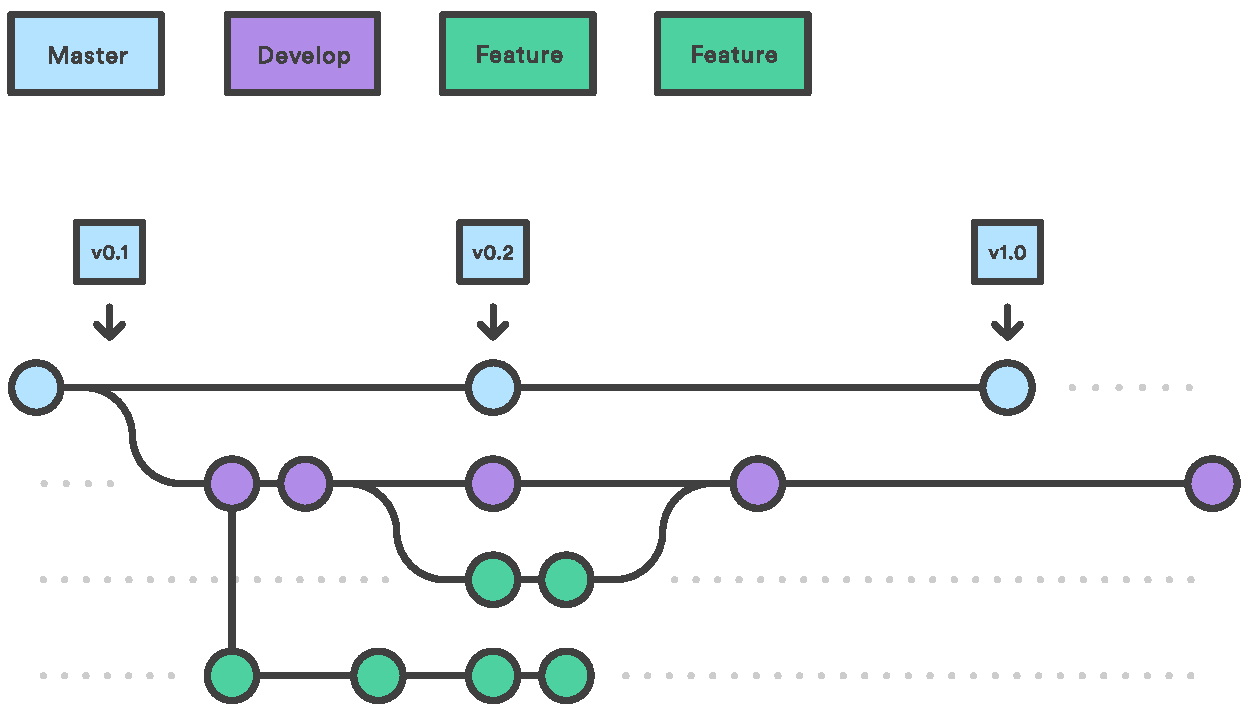
\includegraphics[width=0.8\linewidth]{images/sec3/gitflow.pdf}
        \caption{Schéma illustrant l'interaction entre les différentes branches du flux de travail gitflow}
        \label{fig:gitflow}
    \end{center}
\end{figure}
\subsection{Planification et suivi du projet}
La planification est parmi les phases d'avant-projet. Elle consiste non seulement à délimiter le périmètre temporel du projet, mais aussi à prévoir le déroulement des activités tout au long de la période allouée au stage.

\subsubsection{Diagramme de Gantt}
La figure suivante détaille la planification prévisionnelle du projet (voir figure \ref{fig:gantt}):\\
\begin{figure}[H]
    \begin{center}
        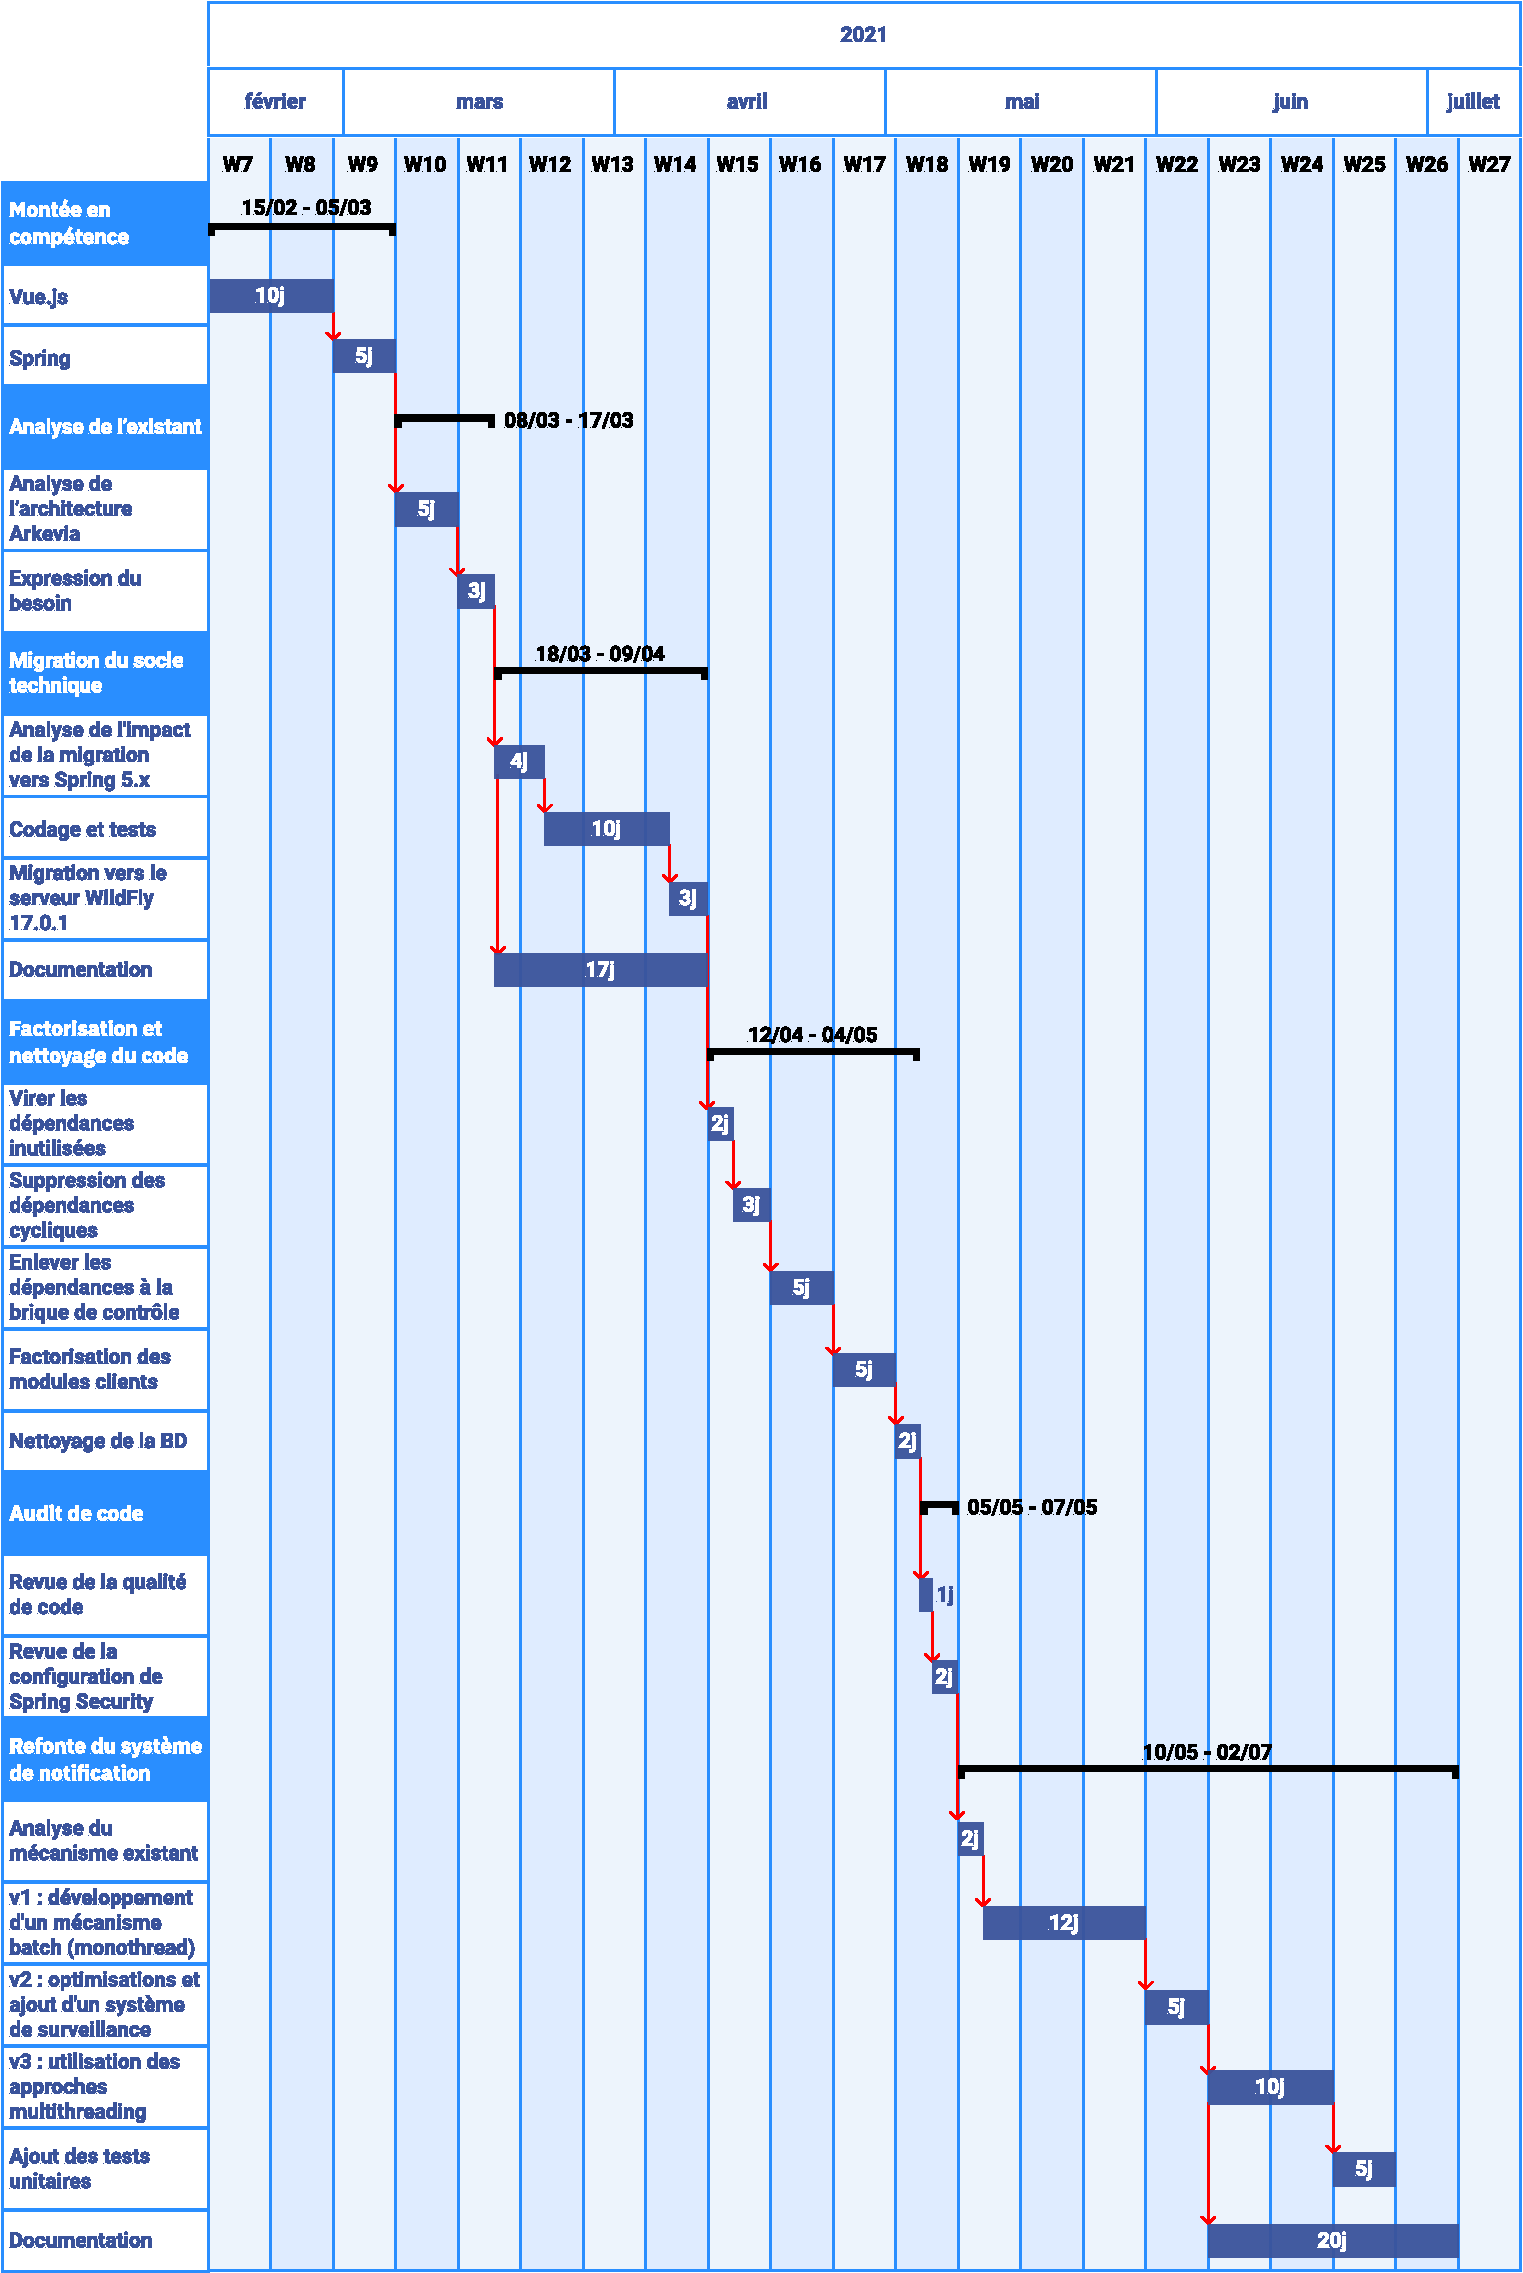
\includegraphics[width=\linewidth]{images/sec3/gantt.pdf}
        \caption{Diagramme de Gantt}
        \label{fig:gantt}
    \end{center}
\end{figure}

\subsection*{Conclusion}
\addcontentsline{toc}{subsection}{Conclusion}
La gestion de projets comme l’on peut le constater s’avère être d’une grande nécessité. Il est nécessaire pour mener à bien un projet de prendre en compte plusieurs dimensions dont toutes ne sont pas forcément quantifiables.\\

Cegedim SRH adopte désormais la méthode Scrum, l'une des méthodes Agile les plus répandues, pour le développement de ses propres solutions. L'Agilité, résolument basée sur l'efficacité et la création de valeur ajoutée, place véritablement clients et éditeurs dans un mode collaboratif avec comme vision un objectif commun.\\

En conséquence, grâce à son expertise avérée de cette méthodologie. Cegedim SRH a pu réduire les délais de conception et de production sans pour autant compromettre la qualité du produit final.
%%%%%%%%%%%%%%%%%%
